% foster_to_cauer.tex
% From the Foster to the Cauer thermal network: the transformation foster_to_cauer()
% pwr-control template (AAA_template_latex_settings); numbers and figures of the worked examples:
% foster_cauer_calc.py (with the module foster_cauer.py), which writes foster_cauer_values.tex
% Compile: pdflatex foster_to_cauer.tex  (twice, for references)
% Rev. 00 - November 2026 - first issue
\documentclass[10pt,a4paper]{scrartcl}
% ===================== PACKAGES =====================
\usepackage[british]{babel}
\usepackage[tmargin=1in, bmargin=1in, lmargin=0.75in, rmargin=0.75in]{geometry}
\usepackage[dvipsnames,table]{xcolor}  % prima di tikz, listings, ecc.

\usepackage{tikz}
\usepackage{graphicx}
\usepackage{pgfplots}
\pgfplotsset{width=12cm, compat=1.9}
\usepackage{setspace}
\usepackage{chemmacros}
\usepackage{chemfig}
\usepackage{esint}
\usepackage{tabularray}
\usepackage{makeidx}
\usepackage{epstopdf}
\usepackage{amssymb}
\usepackage{mathrsfs}
\usepackage{bm}
\usepackage{amsmath}
\usepackage{enumitem}
\usepackage[english]{varioref}
\usepackage{lipsum}
\usepackage{fancyhdr}
\usepackage{float}
\usepackage{empheq}
\usepackage[framemethod=tikz]{mdframed}
\numberwithin{equation}{section}
\usepackage{eso-pic}
\usepackage{calc}
\usepackage{nccmath}
\usepackage{caption}
\usepackage{subcaption}
\usepackage{gensymb}
\usepackage{amsfonts, amsthm, epsfig, epstopdf, titling, url, array}
\usepackage{tabularx}
\usepackage{makecell}
\usepackage{booktabs}
\usepackage{array}
\usepackage{siunitx}
\sisetup{input-digits=0123456789\pi}
\usepackage[symbol]{footmisc}
\usepackage{multicol}
\usepackage{boondox-cal}
\usepackage{blindtext}
\usepackage{changepage}
\usepackage{nomencl}
\usepackage{hyperref}
\usepackage{xurl}
\usepackage{ragged2e}
\usepackage[version=4]{mhchem}  % ← conflitto di opzioni
\usepackage{longtable}
\usepackage{chemformula}
\usetikzlibrary{arrows.meta,positioning,calc}

% ===================== SI UNITS =====================
\DeclareSIUnit\atm{atm}
\DeclareSIUnit{\var}{var}
\DeclareSIUnit{\pu}{p.u.}


% ===================== MATH OPERATORS =====================
\DeclareMathOperator{\rank}{rank}
\DeclareMathOperator{\atantwo}{atan2}
\DeclareMathOperator{\spn}{span}

% ===================== COMMANDS =====================
\newcommand{\abs}[1]{\left|#1\right|}
\newcommand{\sign}{\text{sign}}
\newcommand{\centered}[1]{\begin{tabular}{@{}l@{}} #1 \end{tabular}}

% ===================== COLORS =====================
\definecolor{mycolor1}{rgb}{0.97, 0.97, 0.97}
\definecolor{mycolor2}{rgb}{0.97, 0.97, 0.97}
\definecolor{tableShade}{gray}{0.9}

% ===================== THEOREM ENVIRONMENTS =====================
\theoremstyle{it}
\newtheorem{defn}{Definition}[section]
\newtheorem{assumption}{Assumption}[section]
\newtheorem{thm}{Theorem}[section]
\newtheorem{lemma}{Lemma}[section]
\newtheorem{corollary}{Corollary}[section]
\theoremstyle{definition}
\newtheorem{example}{Example}[section]

% ===================== CUSTOM ENVIRONMENTS =====================
\newenvironment{myitemize_1}{
	\begin{itemize}[topsep=0pt]
		\setlength{\topsep}{2pt}
		\setlength{\itemsep}{2pt}
		\setlength{\parskip}{2pt}
		\setlength{\parsep}{2pt}
	}{\end{itemize}}

\newmdenv[
innerlinewidth=0.5pt,
roundcorner=4pt,
backgroundcolor=mycolor2,
linecolor=mycolor1,
innerleftmargin=6pt,
innerrightmargin=6pt,
innertopmargin=6pt,
innerbottommargin=6pt
]{mybox}

% ===================== TABLE COLUMN TYPES =====================
\newcolumntype{Y}{>{\hsize=2\hsize}X}
\newcolumntype{Z}{>{\centering\arraybackslash\hsize=0.857\hsize}X}

% ===================== SECTION DEPTH =====================
\setcounter{secnumdepth}{3}
\setcounter{tocdepth}{3}

% ===================== PAGE STYLE =====================
\setlength{\headheight}{20pt}
\setlength{\headsep}{20pt}

\pagestyle{fancy}
\fancypagestyle{firstpage}{\rhead{}}
\fancyhead[L]{\slshape\nouppercase{\leftmark}}
\chead{}
\rhead{\includegraphics[height=0.75cm]{../../AAA_template_latex_settings/pwr-control_logo_doc.png}}
\lfoot{\href{http://www.pwr-control.com}{pwr-control.com}}
\cfoot{-\ \thepage\ -}
\rfoot{\textit{}}
\renewcommand{\headrulewidth}{0.4pt}
\renewcommand{\footrulewidth}{0.4pt}


\geometry{
	a4paper,
	top    = 2.5cm,
	bottom = 3.0cm,
	left   = 2.5cm,
	right  = 2.5cm
}

\hypersetup{
	colorlinks = true,
	urlcolor   = blue,
	linkcolor  = black,
	citecolor  = black
}

\pagenumbering{gobble}
% the document sits four levels below the repository root: logo path of settings.tex corrected here
\rhead{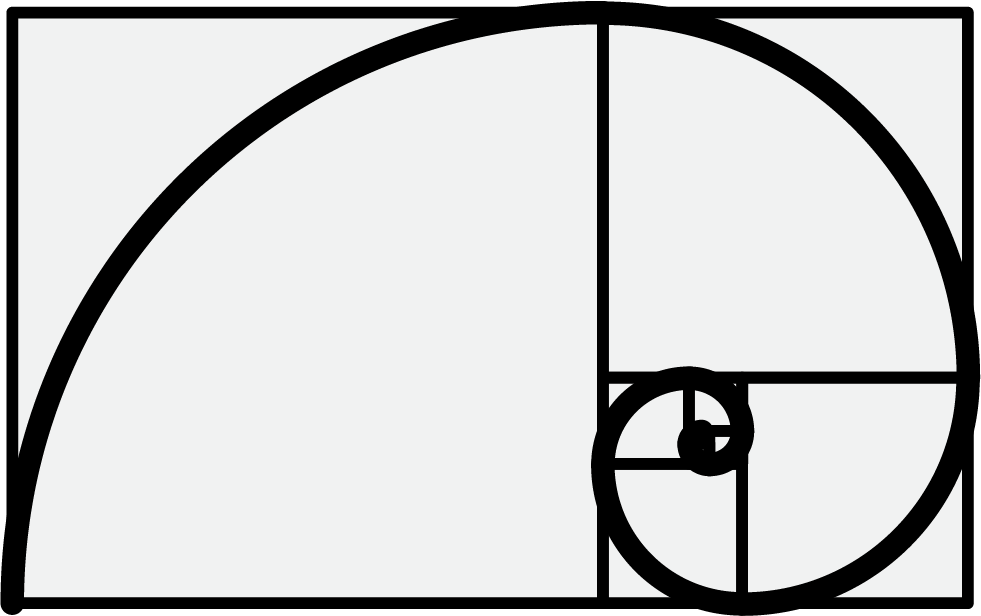
\includegraphics[height=0.75cm]{../../../../AAA_template_latex_settings/pwr-control_logo_doc.png}}
\rfoot{\small Rev.~00}
\geometry{left=2.0cm, right=2.0cm}
\usepackage[european resistors, american inductors]{circuitikz}
\usepackage{listings}

\sisetup{per-mode=symbol,range-phrase={\text{--}},range-units=single}
\setlist{nosep}
\setlength{\parindent}{0pt}
\setlength{\parskip}{3pt}
\allowdisplaybreaks
\captionsetup{font=small,labelfont=bf}
\renewcommand{\topfraction}{0.9}
\renewcommand{\bottomfraction}{0.9}
\renewcommand{\textfraction}{0.05}
\renewcommand{\floatpagefraction}{0.8}
\lstset{language=Python, basicstyle=\ttfamily\footnotesize, columns=fullflexible, keepspaces=true,
  numbers=left, numberstyle=\tiny\color{gray}, numbersep=6pt, xleftmargin=1.5em, frame=lines,
  framerule=0.4pt, rulecolor=\color{gray}, commentstyle=\color{gray!70!black}\itshape,
  keywordstyle=\color{blue!55!black}\bfseries, stringstyle=\color{orange!60!black}, showstringspaces=false}

% --- numbers of the worked examples (generated by foster_cauer_calc.py) ---
% generated by foster_cauer_calc.py: do not edit by hand
\newcommand{\fcddRA}{4.533}
\newcommand{\fcddTA}{0.4406}
\newcommand{\fcddRcA}{0.980}
\newcommand{\fcddCcA}{3.53}
\newcommand{\fcddCfA}{97.2}
\newcommand{\fcddRCcA}{3.46}
\newcommand{\fcddRB}{2.255}
\newcommand{\fcddTB}{0.1045}
\newcommand{\fcddRcB}{1.058}
\newcommand{\fcddCcB}{8.43}
\newcommand{\fcddCfB}{46.3}
\newcommand{\fcddRCcB}{8.92}
\newcommand{\fcddRC}{0.868}
\newcommand{\fcddTC}{0.0092}
\newcommand{\fcddRcC}{3.757}
\newcommand{\fcddCcC}{25.2}
\newcommand{\fcddCfC}{10.6}
\newcommand{\fcddRCcC}{94.71}
\newcommand{\fcddRD}{0.345}
\newcommand{\fcddTD}{0.0022}
\newcommand{\fcddRcD}{2.206}
\newcommand{\fcddCcD}{144.4}
\newcommand{\fcddCfD}{6.38}
\newcommand{\fcddRCcD}{318.68}
\newcommand{\fcddRth}{8.001}
\newcommand{\fcddDelay}{0.56}
\newcommand{\fcddStored}{557}
\newcommand{\fcddThetaA}{8.001}
\newcommand{\fcddThetaB}{7.021}
\newcommand{\fcddThetaC}{5.964}
\newcommand{\fcddThetaD}{2.206}
\newcommand{\fcddCcSum}{181.6}
\newcommand{\fcddCfSum}{160.5}
\newcommand{\fcddCfSeries}{3.53}
\newcommand{\fcddMone}{2.2416}
\newcommand{\fcddErrPoly}{4\times 10^{-16}}
\newcommand{\fcddErrBid}{1\times 10^{-15}}
\newcommand{\fcddErrRt}{3\times 10^{-15}}
\newcommand{\fcddErrZ}{2\times 10^{-15}}
\newcommand{\fcddRpar}{8.03}
\newcommand{\fcddKa}{1.806}
\newcommand{\fcddRsSuma}{14.45}
\newcommand{\fcddRsaA}{1.769}
\newcommand{\fcddRsaB}{1.909}
\newcommand{\fcddRsaC}{6.784}
\newcommand{\fcddRsaD}{3.984}
\newcommand{\fcddCsaB}{4.67}
\newcommand{\fcddCsaC}{14.0}
\newcommand{\fcddCsaD}{80.0}
\newcommand{\fcddKb}{2.241}
\newcommand{\fcddRsSumb}{17.93}
\newcommand{\fcddRsbA}{2.196}
\newcommand{\fcddRsbB}{2.370}
\newcommand{\fcddRsbC}{8.422}
\newcommand{\fcddRsbD}{4.945}
\newcommand{\fcddCsbB}{3.76}
\newcommand{\fcddCsbC}{11.2}
\newcommand{\fcddCsbD}{64.4}
\newcommand{\fcddShareA}{55.4}
\newcommand{\fcdtRA}{3.587}
\newcommand{\fcdtTA}{0.4299}
\newcommand{\fcdtRcA}{0.354}
\newcommand{\fcdtCcA}{2.88}
\newcommand{\fcdtCfA}{119.8}
\newcommand{\fcdtRCcA}{1.02}
\newcommand{\fcdtRB}{0.838}
\newcommand{\fcdtTB}{0.0405}
\newcommand{\fcdtRcB}{0.421}
\newcommand{\fcdtCcB}{4.01}
\newcommand{\fcdtCfB}{48.3}
\newcommand{\fcdtRCcB}{1.69}
\newcommand{\fcdtRC}{0.505}
\newcommand{\fcdtTC}{0.0028}
\newcommand{\fcdtRcC}{1.449}
\newcommand{\fcdtCcC}{32.0}
\newcommand{\fcdtCfC}{5.54}
\newcommand{\fcdtRCcC}{46.41}
\newcommand{\fcdtRD}{0.069}
\newcommand{\fcdtTD}{0.0005}
\newcommand{\fcdtRcD}{2.775}
\newcommand{\fcdtCcD}{110.0}
\newcommand{\fcdtCfD}{7.25}
\newcommand{\fcdtRCcD}{305.37}
\newcommand{\fcdtRth}{4.999}
\newcommand{\fcdtDelay}{0.47}
\newcommand{\fcdtStored}{474}
\newcommand{\fcdtThetaA}{4.999}
\newcommand{\fcdtThetaB}{4.645}
\newcommand{\fcdtThetaC}{4.224}
\newcommand{\fcdtThetaD}{2.775}
\newcommand{\fcdtCcSum}{149.0}
\newcommand{\fcdtCfSum}{181.0}
\newcommand{\fcdtCfSeries}{2.88}
\newcommand{\fcdtMone}{1.5774}
\newcommand{\fcdtErrPoly}{2\times 10^{-16}}
\newcommand{\fcdtErrBid}{9\times 10^{-16}}
\newcommand{\fcdtErrRt}{6\times 10^{-15}}
\newcommand{\fcdtErrZ}{5\times 10^{-15}}
\newcommand{\fcdtRpar}{5.00}
\newcommand{\fcdtKa}{2.000}
\newcommand{\fcdtRsSuma}{10.00}
\newcommand{\fcdtRsaA}{0.708}
\newcommand{\fcdtRsaB}{0.843}
\newcommand{\fcdtRsaC}{2.897}
\newcommand{\fcdtRsaD}{5.550}
\newcommand{\fcdtCsaB}{2.00}
\newcommand{\fcdtCsaC}{16.0}
\newcommand{\fcdtCsaD}{55.0}
\newcommand{\fcdtKb}{2.000}
\newcommand{\fcdtRsSumb}{10.00}
\newcommand{\fcdtRsbA}{0.708}
\newcommand{\fcdtRsbB}{0.843}
\newcommand{\fcdtRsbC}{2.897}
\newcommand{\fcdtRsbD}{5.550}
\newcommand{\fcdtCsbB}{2.00}
\newcommand{\fcdtCsbC}{16.0}
\newcommand{\fcdtCsbD}{55.0}
\newcommand{\fcdtShareA}{50.0}
\newcommand{\fccpP}{15}
\newcommand{\fccpT}{0.5}
\newcommand{\fccpE}{7.5}
\newcommand{\fccpTjI}{98}
\newcommand{\fccpTjC}{101}
\newcommand{\fccpTjF}{141}
\newcommand{\fccpDiff}{41}
\newcommand{\fccpTcC}{14}
\newcommand{\fccpTcF}{44}
\newcommand{\fccpTcFzero}{38}
\newcommand{\fccpQten}{199}
\newcommand{\fccpQend}{33}
\newcommand{\fccpEstored}{6.40}
\newcommand{\fccpEstoredPct}{85}
\newcommand{\fccpRch}{5}
\newcommand{\fccpCbar}{620}
\newcommand{\fcsySaDevF}{20}
\newcommand{\fcsySaAbsF}{20}
\newcommand{\fcsySaDevT}{1.6}
\newcommand{\fcsySaDevX}{-46}
\newcommand{\fcsySaAbsX}{46}
\newcommand{\fcsyScDevF}{19}
\newcommand{\fcsyScAbsF}{19}
\newcommand{\fcsyScDevT}{1.6}
\newcommand{\fcsyScDevX}{-55}
\newcommand{\fcsyScAbsX}{55}
\newcommand{\fcsyNodes}{109}
\newcommand{\fcsyRth}{7.62}
\newcommand{\fcsyRa}{14.2}
\newcommand{\fcsyRc}{17.0}
\newcommand{\fcsyCsi}{2.56}
\newcommand{\fcsyCmo}{28.0}
\newcommand{\fcsyCcu}{171}
\newcommand{\fcsyCtot}{202}
\newcommand{\fcsyModes}{109}
\newcommand{\fcsyCninetyNine}{194}
\newcommand{\fcsyCmax}{2\times 10^{10}}
\newcommand{\fcsyCoFull}{2.56}
\newcommand{\fcsyErrFull}{5\times 10^{-13}}
\newcommand{\fcsyFitThreeErr}{2.36}
\newcommand{\fcsyFitThreeCo}{3.06}
\newcommand{\fcsyFitThreeCsum}{70}
\newcommand{\fcsyFitThreeTmin}{2.40}
\newcommand{\fcsyFitThreeDev}{12.6}
\newcommand{\fcsyFitFourErr}{0.28}
\newcommand{\fcsyFitFourCo}{2.84}
\newcommand{\fcsyFitFourCsum}{106}
\newcommand{\fcsyFitFourTmin}{1.32}
\newcommand{\fcsyFitFourDev}{6.8}
\newcommand{\fcsyFitFiveErr}{0.05}
\newcommand{\fcsyFitFiveCo}{2.78}
\newcommand{\fcsyFitFiveCsum}{115}
\newcommand{\fcsyFitFiveTmin}{0.90}
\newcommand{\fcsyFitFiveDev}{6.0}
\newcommand{\fcsyFitSixErr}{0.01}
\newcommand{\fcsyFitSixCo}{2.75}
\newcommand{\fcsyFitSixCsum}{133}
\newcommand{\fcsyFitSixTmin}{0.66}
\newcommand{\fcsyFitSixDev}{4.7}
\newcommand{\fcsyFRA}{4.764}
\newcommand{\fcsyFTA}{0.3310}
\newcommand{\fcsyRcFA}{0.761}
\newcommand{\fcsyCcFA}{2.84}
\newcommand{\fcsyFRB}{1.900}
\newcommand{\fcsyFTB}{0.0545}
\newcommand{\fcsyRcFB}{1.059}
\newcommand{\fcsyCcFB}{5.80}
\newcommand{\fcsyFRC}{0.708}
\newcommand{\fcsyFTC}{0.0063}
\newcommand{\fcsyRcFC}{2.882}
\newcommand{\fcsyCcFC}{16.7}
\newcommand{\fcsyFRD}{0.251}
\newcommand{\fcsyFTD}{0.0013}
\newcommand{\fcsyRcFD}{2.920}
\newcommand{\fcsyCcFD}{80.5}
\newcommand{\fcsyKa}{1.833}
\newcommand{\fcsyKc}{2.200}
\newcommand{\fcsyHalfZm}{6.76}
\newcommand{\fcsyHalfZc}{7.11}
\newcommand{\fcsyHalfZx}{6.57}
\newcommand{\fcsyHalfZf}{9.48}
\newcommand{\fcsyHalfZi}{6.57}
\newcommand{\fcsyHalfEc}{5.2}
\newcommand{\fcsyHalfEx}{-2.8}
\newcommand{\fcsyHalfEf}{40}
\newcommand{\fcsyHalfEi}{-2.8}
\newcommand{\fcsyMaxEc}{6.8}
\newcommand{\fcsyMinEc}{-0.28}
\newcommand{\fcsyMaxEx}{90}
\newcommand{\fcsyMaxEf}{871}
\newcommand{\fcsyTmaxEf}{1}
\newcommand{\fcsyShortA}{-6}
\newcommand{\fcsyShortB}{-9}
\newcommand{\fcssSaDevF}{20}
\newcommand{\fcssSaAbsF}{20}
\newcommand{\fcssSaDevT}{1.6}
\newcommand{\fcssSaDevX}{-3}
\newcommand{\fcssSaAbsX}{3}
\newcommand{\fcssScDevF}{20}
\newcommand{\fcssScAbsF}{20}
\newcommand{\fcssScDevT}{1.6}
\newcommand{\fcssScDevX}{-3}
\newcommand{\fcssScAbsX}{3}
\newcommand{\fcssNodes}{114}
\newcommand{\fcssRth}{6.98}
\newcommand{\fcssRa}{14.2}
\newcommand{\fcssRc}{14.2}
\newcommand{\fcssCsi}{2.56}
\newcommand{\fcssCmo}{32.0}
\newcommand{\fcssCcu}{171}
\newcommand{\fcssCtot}{206}
\newcommand{\fcssModes}{57}
\newcommand{\fcssCninetyNine}{198}
\newcommand{\fcssCmax}{2\times 10^{1}}
\newcommand{\fcssCoFull}{2.56}
\newcommand{\fcssErrFull}{1\times 10^{-12}}
\newcommand{\fcssFitThreeErr}{3.35}
\newcommand{\fcssFitThreeCo}{3.71}
\newcommand{\fcssFitThreeCsum}{68}
\newcommand{\fcssFitThreeTmin}{1.58}
\newcommand{\fcssFitThreeDev}{14.7}
\newcommand{\fcssFitFourErr}{0.44}
\newcommand{\fcssFitFourCo}{3.21}
\newcommand{\fcssFitFourCsum}{109}
\newcommand{\fcssFitFourTmin}{0.81}
\newcommand{\fcssFitFourDev}{7.4}
\newcommand{\fcssFitFiveErr}{0.05}
\newcommand{\fcssFitFiveCo}{2.98}
\newcommand{\fcssFitFiveCsum}{119}
\newcommand{\fcssFitFiveTmin}{0.52}
\newcommand{\fcssFitFiveDev}{6.2}
\newcommand{\fcssFitSixErr}{0.01}
\newcommand{\fcssFitSixCo}{2.91}
\newcommand{\fcssFitSixCsum}{132}
\newcommand{\fcssFitSixTmin}{0.44}
\newcommand{\fcssFitSixDev}{5.1}
\newcommand{\fcssFRA}{4.870}
\newcommand{\fcssFTA}{0.3488}
\newcommand{\fcssRcFA}{0.376}
\newcommand{\fcssCcFA}{3.21}
\newcommand{\fcssFRB}{1.525}
\newcommand{\fcssFTB}{0.0580}
\newcommand{\fcssRcFB}{0.838}
\newcommand{\fcssCcFB}{7.47}
\newcommand{\fcssFRC}{0.422}
\newcommand{\fcssFTC}{0.0057}
\newcommand{\fcssRcFC}{2.817}
\newcommand{\fcssCcFC}{18.6}
\newcommand{\fcssFRD}{0.159}
\newcommand{\fcssFTD}{0.0008}
\newcommand{\fcssRcFD}{2.945}
\newcommand{\fcssCcFD}{79.6}
\newcommand{\fcssKa}{2.000}
\newcommand{\fcssKc}{2.000}
\newcommand{\fcssHalfZm}{5.98}
\newcommand{\fcssHalfZc}{6.31}
\newcommand{\fcssHalfZx}{5.96}
\newcommand{\fcssHalfZf}{8.72}
\newcommand{\fcssHalfZi}{5.82}
\newcommand{\fcssHalfEc}{5.5}
\newcommand{\fcssHalfEx}{-0.3}
\newcommand{\fcssHalfEf}{46}
\newcommand{\fcssHalfEi}{-2.7}
\newcommand{\fcssMaxEc}{7.4}
\newcommand{\fcssMinEc}{-0.44}
\newcommand{\fcssMaxEx}{1.1}
\newcommand{\fcssMaxEf}{1125}
\newcommand{\fcssTmaxEf}{1}
\newcommand{\fcssShortA}{-12}
\newcommand{\fcssShortB}{-19}
\newcommand{\fcacBadOne}{26}
\newcommand{\fcacPctOne}{24}
\newcommand{\fcacSixOne}{18}
\newcommand{\fcacBidOne}{1\times 10^{-14}}
\newcommand{\fcacBadTwo}{40}
\newcommand{\fcacPctTwo}{36}
\newcommand{\fcacSixTwo}{28}
\newcommand{\fcacBidTwo}{8\times 10^{-15}}
\newcommand{\fcacBadFour}{--}
\newcommand{\fcacPctFour}{--}
\newcommand{\fcacSixFour}{48}
\newcommand{\fcacBidFour}{8\times 10^{-15}}
\newcommand{\fcacBadEight}{--}
\newcommand{\fcacPctEight}{--}
\newcommand{\fcacSixEight}{--}
\newcommand{\fcacBidEight}{7\times 10^{-15}}
\newcommand{\fcacBidMax}{1\times 10^{-14}}
\newcommand{\fcmpDigits}{200}


% --- shorthand ---
\newcommand{\Zth}{Z_\mathrm{th}}
\newcommand{\Zjc}{Z_\mathrm{th(j-c)}}
\newcommand{\Rth}{R_\mathrm{th}}
\newcommand{\Rjc}{R_\mathrm{th(j-c)}}
\newcommand{\Rch}{R_\mathrm{th(c-h)}}
\newcommand{\Tj}{T_\mathrm{j}}
\newcommand{\Tc}{T_\mathrm{c}}
\newcommand{\Rpar}{R_\mathrm{par}}
\newcommand{\diff}{\mathrm{d}}
\newcommand{\lc}{\operatorname{lc}}
\newcommand{\KkW}{\si{\kelvin\per\kilo\watt}}
\newcommand{\JK}{\si{\joule\per\kelvin}}
\newcommand{\ms}{\si{\milli\second}}
\newcommand{\code}[1]{\texttt{#1}}

% =============================================================
%  DOCUMENT DATA (title page: AAA_template_latex_settings/titlepage.tex)
% =============================================================
\newcommand{\DocCategory}{Technical Note}
\newcommand{\DocField}{Power Electronics and Control Systems}
\newcommand{\DocTitle}{%
	{\fontsize{20}{24}\selectfont\bfseries From the Foster to the Cauer} \\[16pt]
	{\fontsize{16}{20}\selectfont\bfseries Thermal Network of a Power Device}
}
\newcommand{\DocSubtitle}{The transformation \texttt{foster\_to\_cauer()}: continued-fraction expansion of the datasheet transient thermal impedance, one ladder per side of a double-side cooled press-pack, numerical accuracy and limits}
\newcommand{\DocAuthor}{Davide Bagnara}
\newcommand{\DocRevision}{00}
\newcommand{\DocDate}{November 2026}
\newcommand{\DocAbstract}{%
Datasheets give the junction-to-case transient thermal impedance of a power device as a Foster network, a sum of exponential terms measured with the case held at a constant temperature. The Foster network reproduces that measurement exactly and nothing else: its nodes are not places in the device, and all the heat leaves it at the case at the instant it is generated. As soon as the case is connected to something that warms up, a contact and a busbar or a heat sink, the Foster network sends the heat there too early and overestimates the junction temperature. The Cauer network, a ladder of resistances and heat capacities from the junction to the case, has the same impedance with the case held constant, but its heat reaches the case with the delay of the heat stored on the way, and its case node can be connected to any external network. This note describes the transformation from one to the other as it is done by the function \texttt{foster\_to\_cauer()}: the Foster sum written as a ratio of two polynomials, the continued-fraction expansion of its inverse, each step with its line of code, why all the elements come out positive, the closed form of the first section, the quantities that any correct conversion preserves and can be checked with. It covers the numerical accuracy of the polynomial expansion, which is at round-off level for the few terms of a datasheet and fails for many closely spaced time constants, and a stable alternative by bidiagonalization; the split of the double-side impedance into one ladder per side with the single-side resistances of the datasheet; and what the ladder does not contain, checked against a press-pack whose layers are known. Worked examples: a \SI{2}{\kilo\volt} rectifier diode and a \SI{1.8}{\kilo\volt} thyristor in press-pack, the diode clamped between two copper bars. The companion Python scripts reproduce every number and figure.
}
\newcommand{\RevisionHistory}{%
	00 & November 2026 & First issue. & \DocAuthor \\
}
\newcommand{\MetaLabelA}{Project Repository}
\newcommand{\MetaValueAUrl}{https://github.com/pwr-control/repositories-documentation.git}
\newcommand{\MetaValueALabel}{repositories-documentation.git}
\newcommand{\MetaLabelB}{Calculation}
\newcommand{\MetaValueB}{Python 3 / NumPy, SciPy (\texttt{foster\_cauer\_calc.py})}

\begin{document}
% =============================================================
%  pwr-control LaTeX template - FRONTESPIZIO
%
%  Da richiamare come prima istruzione dopo \begin{document}:
%      \input{../../AAA_template_latex_settings/titlepage}
%
%  Il documento deve definire prima di \begin{document}:
%      \DocCategory   categoria del documento
%      \DocField      area tecnica
%      \DocTitle      titolo (una o due righe)
%      \DocSubtitle   sottotitolo
%      \DocAuthor     autore/i, separati da virgola
%      \DocRevision   numero di revisione corrente (es. 00)
%      \DocDate       data della revisione corrente
%      \DocAbstract   abstract
%      \RevisionHistory  righe della tabella di revisione, nel formato
%                        Rev. & Date & Description & Authors \\
%      \MetaLabelA \MetaValueAUrl \MetaValueALabel
%      \MetaLabelB \MetaValueB
% =============================================================

\providecommand{\DocCategory}{Technical Research Report}
\providecommand{\DocField}{Power Electronics and Control Systems}
\providecommand{\DocSubtitle}{}
\providecommand{\DocRevision}{00}
\providecommand{\DocAbstract}{}
\providecommand{\RevisionHistory}{%
	\DocRevision & \DocDate & First issue. & \DocAuthor \\
}

\titlepage

% ---- Intestazione centrata ----
\begin{center}
	{\Large\scshape \DocCategory}\\[8pt]
	{\large\scshape \DocField}
\end{center}

\vspace{30pt plus 4pt minus 14pt}
\noindent\rule{\linewidth}{0.8pt}

% ---- Titolo ----
\begin{center}
	\DocTitle
\end{center}

\vspace{4pt}
\noindent\rule{\linewidth}{2.2pt}

% ---- Sottotitolo ----
\begin{center}
	\begin{onehalfspace}
		{\large\itshape \DocSubtitle}
	\end{onehalfspace}
\end{center}

% ---- Authors / Revision / Date ----
\vspace{30pt plus 4pt minus 14pt}

\noindent
\begin{minipage}[t]{0.46\linewidth}
	\raggedright
	\textbf{Authors:}\\[2pt]
	\DocAuthor
\end{minipage}%
\hfill
\begin{minipage}[t]{0.22\linewidth}
	\centering
	\textbf{Revision:}\\[2pt]
	\DocRevision
\end{minipage}%
\hfill
\begin{minipage}[t]{0.30\linewidth}
	\raggedleft
	\textbf{Date:}\\[2pt]
	\DocDate
\end{minipage}

\vspace{10pt}
\noindent\rule{\linewidth}{0.8pt}

% ---- Abstract ----
\vspace{24pt plus 4pt minus 12pt}

\begin{center}
	\begin{minipage}{0.88\linewidth}
		\footnotesize
		\begin{onehalfspace}
			\textbf{Abstract:} \DocAbstract
		\end{onehalfspace}
	\end{minipage}
\end{center}

\vfill

% ---- Revision history ----
\begin{center}
	\begin{minipage}{0.96\linewidth}
		\centering
		{\footnotesize\scshape Revision history}\\[6pt]
		{\footnotesize
			\begin{tabular}{@{}cl>{\raggedright\arraybackslash}p{0.36\linewidth}>{\raggedright\arraybackslash}p{0.28\linewidth}@{}}
				\toprule
				\textbf{Rev.} & \textbf{Date} & \textbf{Description} & \textbf{Authors} \\
				\midrule
				\RevisionHistory
				\bottomrule
			\end{tabular}}
	\end{minipage}
\end{center}

\vspace{18pt plus 4pt minus 10pt}

% ---- Metadati in fondo ----
\noindent
\begin{tabular}{@{} r @{\quad} l @{}}
	\textsc{\MetaLabelA:} & {\href{\MetaValueAUrl}{\MetaValueALabel}} \\[3pt]
	\textsc{\MetaLabelB:} & {\MetaValueB}       \\[3pt]
\end{tabular}

% =============================================================
%  Fine frontespizio
% =============================================================
\newpage
\pagenumbering{arabic}
\setcounter{page}{1}

\tableofcontents
\newpage

%=====================================================================
\section{Scope and results}
\label{sec:scope}
The datasheet of a power device gives the transient thermal impedance from the junction to the case, $\Zjc(t)$: the rise of the junction temperature for a step of one watt of losses, with the case held at a constant temperature. It gives it as a curve and as a table of $n$ pairs $R_i$, $\tau_i$ of the analytical form
\begin{equation}
\Zjc(t) = \sum_{i=1}^{n} R_i \left(1 - e^{-t/\tau_i}\right) ,
\label{eq:zth}
\end{equation}
which is the step response of a Foster network: $n$ cells, each a resistance $R_i$ in parallel with a capacitance $C_i = \tau_i/R_i$, in series from the junction to the case (Fig.~\ref{fig:networks}a).

The Foster network is exact for the test it comes from and only for that test. Its internal nodes are not places in the device, and every cell carries the whole power: the heat leaves the network at the case at the instant it is generated. In a converter the case is not held at a constant temperature; it sits on a contact and a heat sink or a busbar, which warm up. A Foster network connected to them sends the heat into them too early and the junction comes out too hot. The Cauer network, a ladder of heat capacities to the thermal ground and resistances in series (Fig.~\ref{fig:networks}b), has the same impedance when the case is held constant, and it is the lumped model of a one-dimensional heat path: the heat reaches the case with the delay of what is stored on the way, and the case node can be connected to anything.

The function \code{foster\_to\_cauer()} turns the Foster table of a datasheet into the Cauer ladder. It was written for the thermal check of a crowbar stack of press-pack devices clamped between copper bars, where the case is the face of a pole that rests on a bar of finite heat capacity. This note describes what it does and why it works (Secs.~\ref{sec:networks} and~\ref{sec:transform}), how accurate it is and how to do better when it is not (Sec.~\ref{sec:numerics}), how a double-side cooled device is split into one ladder per side (Sec.~\ref{sec:sides}), and what the ladder does and does not contain (Secs.~\ref{sec:examples} and~\ref{sec:synthetic}). Section~\ref{sec:procedure} collects the procedure.

\subsection*{The results in short}
\begin{enumerate}
\item The Foster sum is a ratio of polynomials, $Z(s) = N(s)/D(s)$ with $D = \prod_i (1+s\tau_i)$. The Cauer ladder is the continued-fraction expansion of $Y = 1/Z = D/N$ about $s = \infty$: remove the pole at infinity of the admittance, a capacitance; invert; remove the value at infinity of the impedance, a resistance; invert; repeat $n$ times (Sec.~\ref{sec:cf}). Each element is a ratio of leading coefficients. The function does exactly this with \code{numpy} polynomials (Sec.~\ref{sec:code}).
\item All the elements are positive, and the ladder is unique, because $Z(s)$ is the impedance of an RC network: real negative poles with positive residues (Sec.~\ref{sec:positive}). The first section has a closed form: $C_1 = 1/\sum_i (R_i/\tau_i)$, the initial slope of $\Zjc$, and $R_1 = \bigl(\sum_i R_i/\tau_i\bigr)^2 \big/ \sum_i R_i/\tau_i^2$.
\item A correct conversion keeps $\sum R_k = \sum R_i = \Rjc$, gives $C_1 = 1/\sum (R_i/\tau_i)$, keeps the first moment $\sum_k C_k \theta_k^2 = \sum_i R_i\tau_i$ ($\theta_k$ the resistance from node $k$ to the case), and gives back the $R_i$, $\tau_i$ from the eigenvalues of the ladder (Sec.~\ref{sec:checks}). These are the checks to run on any converted network.
\item For the four terms of a datasheet the polynomial expansion is exact to round-off ($\fcddErrPoly$ for the diode of the examples). It loses digits when the time constants are many and close together: with the time constants spread over one decade the elements are wrong by more than \SI{1}{\percent} from $n = \fcacPctOne$ terms and negative from $n = \fcacBadOne$; over two decades from $n = \fcacPctTwo$ and $n = \fcacBadTwo$ (Fig.~\ref{fig:accuracy}). A bidiagonalization of the eigenvalue form gives the same ladder with products and quotients only, at round-off level for any number of terms (Sec.~\ref{sec:bidiag}).
\item A double-side cooled press-pack has one $\Zjc$ for both sides and one $\Rth$ per side. Each side becomes the same ladder with every $R$ multiplied and every $C$ divided by $k = R_\mathrm{side}/\Rpar$; the junction capacitance $C_1$ is shared. Since $\sum 1/k = 1$, the two ladders in parallel give back the double-side impedance exactly (Sec.~\ref{sec:sides}).
\item For the diode of the examples on two copper bars, a pulse of \SI{\fccpP}{\kilo\watt} for \SI{\fccpT}{\second} raises the junction by \SI{\fccpTjC}{\kelvin} with the Cauer ladders and by \SI{\fccpTjF}{\kelvin} with the Foster network on the bars: \SI{\fccpDiff}{\kelvin} too much. The ladder lets only \SI{\fccpQend}{\percent} of the power into the bars by the end of the pulse; on average the heat leaves the device \SI{\fcddDelay}{\second} after it is generated (Sec.~\ref{sec:onbars}).
\item Checked against a press-pack with known layers, a ladder from a four-term fit as in a datasheet gives the junction temperature on the bars within \SI{\fcsyMinEc}{\percent} and $+\fcsyMaxEc$~\% of the model (high, except for the accuracy of the fit at short pulses), the Foster network $+\fcsyHalfEf$~\% for a pulse of \SI{0.5}{\second} and far more for shorter ones. The ladder of a datasheet fit lacks part of the heat capacity close to the case, which the test with the case held constant hardly sees; the error is on the safe side. The same missing capacity makes the single-side curves of the split ladders up to \SI{\fcsySaDevF}{\percent} too high (Sec.~\ref{sec:synthetic}).
\item More terms are not always better: when the two sides of the device differ, the exact ladder of the double-side curve ends in sections with capacitances up to $\fcsyCmax$~\JK{} that are not material. On the bars they act as a second heat sink and the junction comes out up to \SI{\fcsyMaxEx}{\percent} too cold. A ladder from a fit of few terms has no such sections (Sec.~\ref{sec:missing}).
\end{enumerate}

%=====================================================================
\section{Nomenclature}
\label{sec:nomenclature}
\begin{center}\small
\begin{tabular}{@{}>{$}l<{$}>{\raggedright\arraybackslash}p{6.4cm}>{$}l<{$}>{\raggedright\arraybackslash}p{6.1cm}@{}}
\toprule
\Zjc(t) & transient thermal impedance junction to case, step response to \SI{1}{\watt} & R_i,\ \tau_i & resistance and time constant of the $i$-th Foster term \\
Z(s),\ Y(s) & thermal impedance and admittance in the Laplace domain, $Y = 1/Z$ & C_i^\mathrm{F} & capacitance of a Foster cell, $\tau_i/R_i$ \\
\Rjc & thermal resistance junction to case, $Z(0) = \sum R_i$ & R_k,\ C_k & resistance and heat capacity of the $k$-th section of the Cauer ladder \\
\Rch & contact resistance case to heat sink (or busbar) & \theta_k & resistance from node $k$ of the ladder to the case, $\sum_{j\ge k} R_j$ \\
\Tj,\ \Tc & virtual junction temperature, case temperature & n & number of terms (of sections) \\
p(t) & power dissipated in the device & D(s),\ N(s) & denominator and numerator of $Z(s)$ \\
\lambda_i,\ w_i & poles and residues of $Z$: $1/\tau_i$ and $R_i/\tau_i$ & \lc(\cdot) & leading coefficient of a polynomial \\
\Rpar & parallel of the single-side resistances & k & scale factor of one side, $R_\mathrm{side}/\Rpar$ \\
G,\ \mathbf{C} & conductance matrix and capacitance matrix of a network & M & symmetric matrix $\mathbf{C}^{-1/2} G\, \mathbf{C}^{-1/2}$ \\
\bottomrule
\end{tabular}
\end{center}
Thermal quantities follow the electrical analogy: temperature is a voltage, heat flow a current, the thermal ground is the reference temperature. All temperatures are rises above the initial temperature, which is also the temperature of an ideal heat sink. Resistances are given in \KkW{} as in the datasheets, capacitances in \JK.

%=====================================================================
\section{The two networks}
\label{sec:networks}

\subsection{What the datasheet measures}
The transient thermal impedance is measured with a step of power in the device and the case held at a constant temperature, usually on a water-cooled heat sink; the junction temperature is the virtual one, read from a temperature-sensitive electrical parameter. The curve covers a time window of a few decades, typically \SI{1}{\milli\second} to \SI{10}{\second} or more, and the table \eqref{eq:zth} is a fit of it with a few exponential terms. For a press-pack the datasheet gives the curve and the table for double-side cooling, and the steady-state resistance also for anode-side and cathode-side cooling.

Two facts follow and matter for the rest of the note. The table is a fit: other sets of $R_i$, $\tau_i$, with more or fewer terms, fit the same curve within its accuracy, and outside the window of the measurement the table is an extrapolation. And the table describes one boundary condition, the case held at a constant temperature; any other boundary condition is outside what was measured.

\subsection{Foster network}
In the Laplace domain the table \eqref{eq:zth} is
\begin{equation}
Z(s) = \sum_{i=1}^{n} \frac{R_i}{1 + s\tau_i} = \sum_{i=1}^{n} \frac{w_i}{s + \lambda_i} , \qquad \lambda_i = \frac{1}{\tau_i} , \quad w_i = \frac{R_i}{\tau_i} ,
\label{eq:zfoster}
\end{equation}
the sum of the impedances of $n$ parallel cells $R_i \parallel C_i^\mathrm{F}$ with $C_i^\mathrm{F} = \tau_i/R_i$, in series (Fig.~\ref{fig:networks}a). Three properties of this network decide how it can be used.
\begin{itemize}
\item The cells are in series, so each carries the whole power $p(t)$: the heat flow out of the last cell into the case is $p(t)$ at every instant. Nothing is stored on the way, as far as the case can tell.
\item The temperature of an internal node is the sum of the drops of the cells before it. It is not the temperature of any layer of the device, and the capacitances $C_i^\mathrm{F}$ are not heat capacities of anything: they sit across the resistances, not between a node and the thermal ground.
\item The junction temperature is $\Tj(t) = \Tc(t) + \int_0^t \Zjc'(t-u)\,p(u)\,\diff u$ whatever happens to the case. With the case held constant this is right. With the case on a heat sink that warms up, the heat sink is driven by $p(t)$ itself instead of by the heat that actually reaches it, which arrives later and smoothed.
\end{itemize}
The third point is the usual sum of a junction-case and a case-ambient impedance, each driven by the full power. It is a valid upper bound in the examples of this note and in common use for that reason, but it can be far from the real temperature (Secs.~\ref{sec:onbars} and~\ref{sec:synthetic}).

\begin{figure}[htb]
\centering
\begin{circuitikz}[scale=0.82, transform shape, european resistors]
\begin{scope}
\node[anchor=west] at (-0.6,2.2) {\textbf{(a)} Foster network};
\draw (0,-1.6) node[ground]{} to[I, l=$p(t)$, invert] (0,0);
\draw (0,0) node[circ]{} node[above left]{$\Tj$} -- (0.5,0);
\foreach \i/\x in {1/0.5,2/2.7,3/4.9,4/7.1} {
  \draw (\x,0) -- (\x,0.6) to[R, l=$R_\i$] (\x+1.7,0.6) -- (\x+1.7,0);
  \draw (\x,0) -- (\x,-0.6) to[C, l_=$C^\mathrm{F}_\i$] (\x+1.7,-0.6) -- (\x+1.7,0);
}
\draw (2.2,0) -- (2.7,0); \draw (4.4,0) -- (4.9,0); \draw (6.6,0) -- (7.1,0);
\draw (8.8,0) -- (9.6,0) node[circ]{} node[above]{$\Tc$} -- (10.2,0) to[V, l=$\Tc$ held, invert] (10.2,-1.6) node[ground]{};
\end{scope}
\begin{scope}[yshift=-5.0cm]
\node[anchor=west] at (-0.6,2.0) {\textbf{(b)} Cauer network};
\draw (0,-1.6) node[ground]{} to[I, l=$p(t)$, invert] (0,0);
\draw (0,0) node[circ]{} node[above left]{$\Tj$} -- (1.6,0) node[circ]{};
\draw (1.6,0) to[C, l_=$C_1$] (1.6,-1.6) node[ground]{};
\draw (1.6,0) to[R, l=$R_1$] (3.6,0) node[circ]{};
\draw (3.6,0) to[C, l_=$C_2$] (3.6,-1.6) node[ground]{};
\draw (3.6,0) to[R, l=$R_2$] (5.6,0) node[circ]{};
\draw (5.6,0) to[C, l_=$C_3$] (5.6,-1.6) node[ground]{};
\draw (5.6,0) to[R, l=$R_3$] (7.6,0) node[circ]{};
\draw (7.6,0) to[C, l_=$C_4$] (7.6,-1.6) node[ground]{};
\draw (7.6,0) to[R, l=$R_4$] (9.6,0) node[circ]{} node[below left]{$\Tc$} -- (10.2,0) to[V, l=$\Tc$ held, invert] (10.2,-1.6) node[ground]{};
\draw[densely dashed, gray] (9.6,0) -- (9.6,0.9) node[above, black, font=\small]{or any external network};
\end{scope}
\end{circuitikz}
\caption{The two networks of a four-term $\Zjc$. (a) Foster: cells in series, each carrying the whole power; only the junction node has a physical meaning. (b) Cauer: heat capacities to the thermal ground and resistances in series, a lumped one-dimensional heat path from the junction to the case. With the case held at a constant temperature the two have the same impedance; only the ladder can be connected to an external network at the case.}
\label{fig:networks}
\end{figure}

\subsection{Cauer network}
The Cauer network (Fig.~\ref{fig:networks}b) is a ladder: node 1, the junction, with the capacitance $C_1$ to the thermal ground, the resistance $R_1$ to node 2 with $C_2$, and so on to $R_n$, which ends at the case. It is the lumped model of a slab-like heat path: $C_k$ is the heat capacity of a slice of the path, $R_k$ the resistance between two slices. Its impedance, with the case held constant, is the continued fraction
\begin{equation}
Z(s) = \cfrac{1}{sC_1 + \cfrac{1}{R_1 + \cfrac{1}{sC_2 + \cfrac{1}{R_2 + \cdots + \cfrac{1}{sC_n + \cfrac{1}{R_n}}}}}} .
\label{eq:zcauer}
\end{equation}
Given $Z(s)$ of the form \eqref{eq:zfoster}, the ladder with the same impedance exists, has positive elements and is unique (Sec.~\ref{sec:positive}). With the case held constant the two networks cannot be told apart from the junction: same $\Zjc(t)$, same junction temperature for any power waveform. They differ inside, and that difference shows as soon as the case is not held constant.
\begin{itemize}
\item In the ladder the heat reaches the case only after it has warmed the capacitances on the way. For a step of power the heat flow into the case starts from zero; the heat stored in the device in steady state is $p\sum_k C_k\theta_k$, where $\theta_k = \sum_{j\geq k} R_j$ is the resistance from node $k$ to the case. That same sum is the mean delay with which the heat leaves the case after it is generated.
\item The case node is a node like the others: a contact resistance, a heat sink, a busbar or a second device can be connected there, and the network of the whole stack is again a network of capacitances to ground and resistances, solved by any circuit or thermal solver.
\item The ladder is not the device. It is the one-dimensional lumped path that has the measured impedance; how close its sections come to the real layers is the subject of Sec.~\ref{sec:synthetic}.
\end{itemize}

%=====================================================================
\section{The transformation}
\label{sec:transform}

\subsection{The Foster sum as a ratio of polynomials}
Over a common denominator, \eqref{eq:zfoster} is
\begin{equation}
Z(s) = \frac{N(s)}{D(s)} , \qquad D(s) = \prod_{i=1}^{n} (1 + s\tau_i) , \qquad N(s) = \sum_{k=1}^{n} R_k \prod_{j \neq k} (1 + s\tau_j) .
\label{eq:nd}
\end{equation}
$D$ has degree $n$, $N$ degree $n-1$. The admittance $Y = D/N$ therefore grows like $s$ at high frequency: it has a pole at infinity, which is the capacitance $C_1$ of the junction node.

\subsection{Continued fraction}
\label{sec:cf}
Write the admittance at step $k$ as $Y_k = D_k/N_k$ with $\deg D_k = \deg N_k + 1$; at the start $D_1 = D$ and $N_1 = N$. One step removes a capacitance and a resistance:
\begin{align}
C_k &= \frac{\lc D_k}{\lc N_k} , & P_k &= D_k - s\,C_k\, N_k , & Y_k - sC_k &= \frac{P_k}{N_k} , \label{eq:stepC}\\
R_k &= \frac{\lc N_k}{\lc P_k} , & Q_k &= N_k - R_k\, P_k , & \frac{N_k}{P_k} - R_k &= \frac{Q_k}{P_k} , \label{eq:stepR}
\end{align}
and the next admittance is $Y_{k+1} = P_k/Q_k$, that is $D_{k+1} = P_k$, $N_{k+1} = Q_k$. Here $\lc$ is the leading coefficient, the coefficient of the highest power of $s$.

The degrees explain each step. $D_k$ and $sN_k$ have the same degree, and $C_k$ is chosen so that their leading terms cancel: $P_k$ has the degree of $N_k$, and $P_k/N_k$ has a finite value at infinity. Its inverse $N_k/P_k$ is an impedance with a finite value at infinity, $R_k$; removing it cancels again the leading term, and $Q_k$ has one degree less than $P_k$, so that $P_k/Q_k$ again has a pole at infinity. Each step lowers both degrees by one; after $n$ steps $N_n$ is a constant, $P_n$ is a constant and $Q_n = 0$. In the ladder this reads
\begin{equation}
Y_k = sC_k + \cfrac{1}{R_k + \cfrac{1}{Y_{k+1}}} ,
\end{equation}
which, repeated, is \eqref{eq:zcauer}: $C_k$ is the capacitance from node $k$ to ground, $R_k$ the resistance to node $k+1$, and $1/Y_{k+1}$ the impedance of the rest of the ladder seen from node $k+1$.

\subsection{Why the elements are positive}
\label{sec:positive}
$Z(s)$ in \eqref{eq:zfoster} has simple poles on the negative real axis with positive residues $w_i$, is zero at infinity and positive at zero: it is the driving-point impedance of an RC network. Such functions have three properties used here \cite{foster1924,cauer1926,guillemin1957}: their zeros and poles are real, simple and alternate on the negative real axis; the inverse of an RC impedance is an RC admittance, which has the form $Y(s) = s\,c_\infty + g_0 + \sum_j g_j\, s/(s+\sigma_j)$ with non-negative coefficients; and what is left after removing from an RC function a pole at infinity, or its value at infinity, is again an RC function, with one pole less.

From the first expansion of $Z$ about infinity,
\begin{equation}
Z(s) = \frac{1}{s}\sum_i w_i - \frac{1}{s^2}\sum_i \frac{w_i}{\tau_i} + O\!\left(s^{-3}\right) , \qquad
Y(s) = \frac{s}{\sum_i w_i} + \frac{\sum_i w_i/\tau_i}{\bigl(\sum_i w_i\bigr)^2} + O\!\left(s^{-1}\right) ,
\end{equation}
the first section comes out in closed form,
\begin{equation}
C_1 = \frac{1}{\sum_i R_i/\tau_i} , \qquad R_1 = \frac{\bigl(\sum_i R_i/\tau_i\bigr)^2}{\sum_i R_i/\tau_i^2} ,
\label{eq:first}
\end{equation}
both positive. $C_1$ is the inverse of the initial slope of $\Zjc(t)$: for $t$ much shorter than the shortest $\tau_i$, $\Zjc(t) \approx t/C_1$, and all the networks with this $Z(s)$ behave at the start as one capacitance $C_1$. It is the effective heat capacity of the active clamping note of this repository \cite{activeclamping}, and the series combination of the Foster capacitances, $1/C_1 = \sum_i 1/C_i^\mathrm{F}$.

Then $Y - sC_1$ is an RC admittance without pole at infinity and with a positive value there, $1/R_1$; its inverse minus $R_1$ is an RC impedance zero at infinity, of the same form as $Z$ with $n-1$ poles; and the argument repeats. All the $C_k$ and $R_k$ are positive, there are exactly $n$ of each, and since each step is forced the ladder is unique. This is Cauer's first canonical form \cite{cauer1926}.

\subsection{The function, line by line}
\label{sec:code}
The function takes the Foster table and returns the ladder, $R$ in the same unit as the table and $C$ in J/K when $R$ is in K/W and $\tau$ in seconds. Polynomials are \code{numpy} arrays of coefficients in descending powers of $s$, so the leading coefficient is the element \code{[0]}.
\begin{lstlisting}
def foster_to_cauer(R, tau):
    n = len(R)
    D = np.array([1.0])
    for ti in tau:
        D = np.polymul(D, [ti, 1.0])                              # D = prod (tau_i s + 1)
    N = np.zeros(1)
    for k in range(n):
        term = np.array([R[k]])
        for j in range(n):
            if j != k:
                term = np.polymul(term, [tau[j], 1.0])
        N = np.polyadd(N, term)                                    # N = sum R_k prod_{j!=k} (tau_j s + 1)
    num, den = D, N                      # Y(s) = num / den, deg(num) = deg(den) + 1
    Cs, Rs = [], []
    for _ in range(n):
        C = num[0] / den[0]
        rem = np.polysub(num, np.polymul([C, 0.0], den))[1:]      # Y - s C   (leading term cancels)
        Rk = den[0] / rem[0]
        rem2 = np.polysub(den, Rk * rem)[1:]                       # Z - R     (leading term cancels)
        Cs.append(C); Rs.append(Rk)
        num, den = rem, rem2
    return np.array(Rs), np.array(Cs)
\end{lstlisting}
\begin{itemize}
\item Lines 3--12 build $D$ and $N$ of \eqref{eq:nd}; \code{[ti, 1.0]} is the polynomial $\tau_i s + 1$.
\item Line 13: \code{num}, \code{den} are $D_k$, $N_k$ of the current admittance.
\item Line 16 is $C_k = \lc D_k/\lc N_k$ of \eqref{eq:stepC}; line 17 forms $P_k = D_k - sC_kN_k$ (\code{[C, 0.0]} is the polynomial $C_k s$) and drops its first coefficient, which is zero in exact arithmetic and a round-off residue in floating point.
\item Line 18 is $R_k = \lc N_k/\lc P_k$ of \eqref{eq:stepR}; line 19 forms $Q_k = N_k - R_kP_k$ and drops its first coefficient for the same reason.
\item Line 21 passes to the next section, $D_{k+1} = P_k$, $N_{k+1} = Q_k$. At the last pass \code{rem2} is empty: $Q_n = 0$.
\end{itemize}
The first coefficient is dropped, not tested: the function relies on the theory for the cancellation, and in floating point it never checks how large the residue was. This is harmless for the few terms of a datasheet and is where the accuracy goes when the terms are many (Sec.~\ref{sec:numerics}). The order of the input terms does not matter, since $D$ and $N$ are symmetric in them.

\subsection{Back from the ladder to the table}
\label{sec:inverse}
The inverse transformation is a check and a tool: it turns a ladder into the Foster table that a simulator or a datasheet comparison needs. The node equations of the ladder with the case held constant are $\mathbf{C}\,\dot{\boldsymbol\theta} = -G\boldsymbol\theta + \mathbf{e}_1 p$, with $\mathbf{C} = \operatorname{diag}(C_k)$ and $G$ tridiagonal, $G_{kk} = 1/R_{k-1} + 1/R_k$ ($1/R_0 = 0$) and $G_{k,k+1} = G_{k+1,k} = -1/R_k$. With the symmetric matrix $M = \mathbf{C}^{-1/2}G\,\mathbf{C}^{-1/2} = Q\Lambda Q^\mathsf{T}$,
\begin{equation}
Z(s) = \mathbf{e}_1^\mathsf{T}(s\mathbf{C} + G)^{-1}\mathbf{e}_1 = \frac{1}{C_1}\sum_{i=1}^{n} \frac{q_{1i}^2}{s + \lambda_i}
\quad\Longrightarrow\quad
\tau_i = \frac{1}{\lambda_i} , \qquad R_i = \frac{q_{1i}^2}{C_1\lambda_i} ,
\label{eq:eig}
\end{equation}
where $q_{1i}$ is the first component of the $i$-th unit eigenvector. The Foster time constants are the eigenvalues of the ladder, not the products $R_kC_k$ of its sections. Comparing \eqref{eq:eig} with \eqref{eq:zfoster} gives again $C_1 = 1/\sum_i w_i$, since the $q_{1i}^2$ add up to one.

\subsection{What every correct conversion preserves}
\label{sec:checks}
Four quantities depend on $Z(s)$ alone and can be computed on both sides of a conversion:
\begin{enumerate}
\item the resistance, $Z(0)$: $\sum_k R_k = \sum_i R_i = \Rjc$;
\item the junction capacitance \eqref{eq:first}: $C_1 = 1/\sum_i (R_i/\tau_i)$, also $1/\sum_i (1/C_i^\mathrm{F})$;
\item the first moment, $-Z'(0)$, which is the area between $\Rjc$ and the curve $\Zjc(t)$: on the Foster side $\sum_i R_i\tau_i$; on the ladder side $\boldsymbol\theta^\mathsf{T}\mathbf{C}\,\boldsymbol\theta = \sum_k C_k\theta_k^2$, with $\boldsymbol\theta = G^{-1}\mathbf{e}_1$ the steady-state node temperatures at one watt, $\theta_k = \sum_{j\ge k} R_j$;
\item the poles and residues: the eigenvalues and first eigenvector components of the ladder \eqref{eq:eig} give back the $\tau_i$ and $R_i$.
\end{enumerate}
The total capacitance is not among them: $\sum_k C_k$ and $\sum_i C^\mathrm{F}_i$ are different numbers ($\fcddCcSum$ and $\fcddCfSum$~\JK{} for the diode of Sec.~\ref{sec:examples}), and neither is the heat capacity of the device (Sec.~\ref{sec:missing}).

%=====================================================================
\section{Numerical accuracy}
\label{sec:numerics}

\subsection{Where the polynomial expansion loses digits}
Every step of \eqref{eq:stepC}--\eqref{eq:stepR} subtracts two polynomials whose leading terms are equal by construction, and the information is in what is left. The coefficients of $D$ and $N$ are elementary symmetric functions of the $\tau_i$; working with them is working with the moments $\sum_i w_i/\tau_i^m$ of the time-constant spectrum, as \eqref{eq:first} shows for the first section. The map from moments to a continued fraction is the classical route to orthogonal polynomials, and it is ill-conditioned: its condition number grows exponentially with the number of terms, the faster the closer the time constants are to each other \cite{gautschi2004}. When the time constants are few and far apart, as in a datasheet, each coefficient is dominated by a different product of time constants and the subtractions lose few digits; when they are many and close, the remainders become differences of nearly equal numbers and the digits run out. A second limit is the range of double precision: the leading coefficient of $D$ is $\prod_i\tau_i$, which underflows for a hundred terms down to $10^{-8}$~s.

\subsection{A stable alternative: bidiagonalization}
\label{sec:bidiag}
The eigenvalue form \eqref{eq:eig} gives a way that never builds a polynomial. For the ladder, $G = E\,\operatorname{diag}(1/R_k)\,E^\mathsf{T}$, with $E$ the lower bidiagonal matrix with $1$ on the diagonal and $-1$ below it (the incidence matrix of the resistances, the last one going to the case). Hence
\begin{equation}
M = BB^\mathsf{T} , \qquad B = \mathbf{C}^{-1/2} E\, \operatorname{diag}(R_k)^{-1/2} , \qquad B_{kk} = \frac{1}{\sqrt{C_kR_k}} , \quad B_{k+1,k} = -\frac{1}{\sqrt{C_{k+1}R_k}} ,
\end{equation}
so $B$ is the lower bidiagonal factor of $M$, whose singular values are $\sqrt{\lambda_i}$. Given the poles $\lambda_i$ and the vector $\mathbf{u}$ of first eigenvector components, $u_i = \sqrt{w_i C_1}$, the Golub--Kahan bidiagonalization of $A = \operatorname{diag}\bigl(\sqrt{\lambda_i}\bigr)$ started from $\mathbf{u}$ \cite{golubkahan1965,paige1982} returns the bidiagonal matrix with diagonal $\alpha_k$ and subdiagonal $\beta_{k+1}$ such that $BB^\mathsf{T}$ has eigenvalues $\lambda_i$ and eigenvectors with first components $u_i$. The signs of the entries do not affect the impedance, and the ladder follows with products and quotients of positive numbers only:
\begin{equation}
C_1 = \frac{1}{\sum_i w_i} , \qquad R_k = \frac{1}{\alpha_k^2\, C_k} , \qquad C_{k+1} = \frac{1}{\beta_{k+1}^2\, R_k} .
\label{eq:bidiag}
\end{equation}
With full reorthogonalization the bidiagonalization works on the spectrum directly and never forms the moments; in the tests of Fig.~\ref{fig:accuracy} its ladder is at round-off level for any number of terms. It is the same idea as the reconstruction of a Jacobi matrix from spectral data \cite{gragg1984}. The module implements it as \code{foster\_to\_cauer\_bidiag()}, next to the function of Sec.~\ref{sec:code} unchanged and to a reference with \fcmpDigits{} significant digits, \code{foster\_to\_cauer\_mp()}, which repeats the same polynomial steps in decimal arithmetic.

\subsection{How many terms the polynomial expansion takes}
Figure~\ref{fig:accuracy} compares the two algorithms with the reference for $n$ equal resistances and time constants spaced evenly on a logarithmic scale over one to eight decades. The polynomial expansion is at round-off level for the four to six terms of a datasheet whatever their spread. It degrades with the density of the time constants, not with their spread: over one decade the error passes $10^{-6}$ at $n = \fcacSixOne$, \SI{1}{\percent} at $n = \fcacPctOne$, and from $n = \fcacBadOne$ some elements are negative; over two decades the same happens at $n = \fcacSixTwo$, $\fcacPctTwo$ and $\fcacBadTwo$; over four decades the error passes $10^{-6}$ at $n = \fcacSixFour$; over eight decades it stays below that up to sixty terms. The bidiagonalization stays below $\fcacBidMax$ everywhere.

So the function of Sec.~\ref{sec:code} is right for what it was written for, a datasheet table. A fit with many terms per decade, as in the structure-function analysis of a measured curve \cite{szekely1997,jesd5114}, needs the bidiagonalization or extended precision; the synthetic device of Sec.~\ref{sec:synthetic}, with $\fcsyModes$ terms, is an example where the polynomial expansion returns negative elements.

\begin{figure}[htb]
\centering
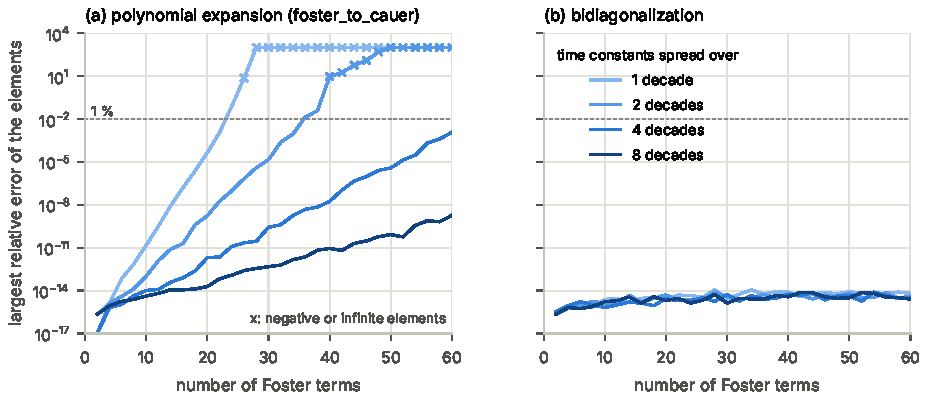
\includegraphics[width=\textwidth]{figures/fig_accuracy.pdf}
\caption{Largest relative error of the ladder elements against the \fcmpDigits-digit reference, for $n$ Foster terms of equal resistance with time constants evenly spaced on a logarithmic scale over one to eight decades. (a) Polynomial expansion, the function \code{foster\_to\_cauer()}: the error grows with the density of the time constants; crosses mark negative or infinite elements (errors above $10^3$ drawn at $10^3$). (b) Bidiagonalization, \eqref{eq:bidiag}: round-off level throughout.}
\label{fig:accuracy}
\end{figure}

%=====================================================================
\section{Double-side cooling: one ladder per side}
\label{sec:sides}

\subsection{The split}
A press-pack is cooled through both poles, and its two cases may see different external networks: different contacts, a bar on one side and a heat sink on the other, a neighbouring device. The datasheet gives one impedance for both sides together, $Z(s)$, and the steady-state resistances for the anode side and the cathode side alone, $R_\mathrm{a}$ and $R_\mathrm{c}$. The split used in the thermal model takes the ladder of $Z$ and makes one copy per side, scaled:
\begin{equation}
\Rpar = \left(\frac{1}{R_\mathrm{a}} + \frac{1}{R_\mathrm{c}}\right)^{-1} , \qquad k_\mathrm{a} = \frac{R_\mathrm{a}}{\Rpar} , \quad k_\mathrm{c} = \frac{R_\mathrm{c}}{\Rpar} ; \qquad
\text{side } x\!: \ R_k\, k_x \ (k = 1\ldots n) , \quad \frac{C_k}{k_x} \ (k = 2\ldots n) ,
\label{eq:split}
\end{equation}
with the junction node and its capacitance $C_1$ shared by the two sides (Fig.~\ref{fig:split}).

Multiplying every resistance by $k$ and dividing every capacitance by $k$ multiplies every impedance of the ladder by $k$, at every frequency. Let $Z'(s)$ be the impedance of the ladder of $Z$ seen from the junction without $C_1$; the two scaled copies in parallel have the impedance
\begin{equation}
\left(\frac{1}{k_\mathrm{a}Z'} + \frac{1}{k_\mathrm{c}Z'}\right)^{-1} = \frac{Z'}{1/k_\mathrm{a} + 1/k_\mathrm{c}} = Z' ,
\qquad\text{since}\qquad \frac{1}{k_\mathrm{a}} + \frac{1}{k_\mathrm{c}} = \Rpar\left(\frac{1}{R_\mathrm{a}} + \frac{1}{R_\mathrm{c}}\right) = 1 .
\end{equation}
With $C_1$ in parallel, this is $Z(s)$: with both cases held at the same temperature the split network has exactly the double-side impedance of the datasheet, and the sum of the capacitances of the two copies is the capacitance of the ladder. In steady state the share of the heat that leaves through the anode is $1/k_\mathrm{a} = R_\mathrm{c}/(R_\mathrm{a}+R_\mathrm{c})$.

Only the ratio $R_\mathrm{a}/R_\mathrm{c}$ enters the split. If $\sum R_i$ of the table and $\Rpar$ of the single-side values differ slightly, as they usually do in a datasheet, the single-side resistances of the split ladders are $k_x\sum R_i$, not exactly $R_x$; the double-side impedance is kept.

\begin{figure}[htb]
\centering
\begin{circuitikz}[scale=0.8, transform shape, european resistors]
% junction, shared capacitance, power
\draw (0,-1.4) node[ground]{} to[I, l=$p(t)$, invert] (0,0);
\draw (0,0) node[circ]{} node[above left]{$\Tj$} -- (1.4,0) node[circ]{};
\draw (1.4,0) to[C, l_=$C_1$] (1.4,-1.4) node[ground]{};
\draw (1.4,0) -- (1.4,3.0) -- (2.2,3.0);
\draw (1.4,0) -- (2.2,0);
% anode side, upper row
\draw (2.2,3.0) to[R, l=$R_1k_\mathrm{a}$] (4.2,3.0) node[circ]{};
\draw (4.2,3.0) to[C, l_=$C_2/k_\mathrm{a}$] (4.2,1.6) node[ground]{};
\draw (4.2,3.0) to[R, l=$R_2k_\mathrm{a}$] (6.4,3.0) node[circ]{};
\draw (6.4,3.0) to[C, l_=$C_3/k_\mathrm{a}$] (6.4,1.6) node[ground]{};
\draw (6.4,3.0) to[R, l=$R_3k_\mathrm{a}$] (8.6,3.0) node[circ]{};
\draw (8.6,3.0) to[C, l_=$C_4/k_\mathrm{a}$] (8.6,1.6) node[ground]{};
\draw (8.6,3.0) to[R, l=$R_4k_\mathrm{a}$] (10.8,3.0) node[circ]{} node[below=3pt]{case a};
\draw (10.8,3.0) to[R, l=$\Rch$] (13.0,3.0) node[circ]{};
\draw (13.0,3.0) to[C, l=bar or heat sink] (13.0,1.6) node[ground]{};
% cathode side, lower row
\draw (2.2,0) to[R, l=$R_1k_\mathrm{c}$] (4.2,0) node[circ]{};
\draw (4.2,0) to[C, l_=$C_2/k_\mathrm{c}$] (4.2,-1.4) node[ground]{};
\draw (4.2,0) to[R, l=$R_2k_\mathrm{c}$] (6.4,0) node[circ]{};
\draw (6.4,0) to[C, l_=$C_3/k_\mathrm{c}$] (6.4,-1.4) node[ground]{};
\draw (6.4,0) to[R, l=$R_3k_\mathrm{c}$] (8.6,0) node[circ]{};
\draw (8.6,0) to[C, l_=$C_4/k_\mathrm{c}$] (8.6,-1.4) node[ground]{};
\draw (8.6,0) to[R, l=$R_4k_\mathrm{c}$] (10.8,0) node[circ]{} node[below=3pt]{case c};
\draw (10.8,0) to[R, l=$\Rch$] (13.0,0) node[circ]{};
\draw (13.0,0) to[C, l=bar or heat sink] (13.0,-1.4) node[ground]{};
\end{circuitikz}
\caption{The ladder of the double-side impedance split into one ladder per side, \eqref{eq:split}: the junction node and $C_1$ are shared; each side, anode above and cathode below, is the rest of the ladder with $R\times k$ and $C/k$ and ends at its own case node, connected to its own external network (here a contact resistance and a lumped busbar or heat sink).}
\label{fig:split}
\end{figure}

\subsection{What the split assumes}
The split is exact for the double-side impedance and for the single-side resistances, and an assumption for everything else. It assumes that the two heat paths have the same shape and differ only by a scale factor: the same distribution of resistance and capacitance along the path, more of both on one side. In a real press-pack they differ in the layers (a molybdenum disc alloyed to the silicon on one side, a free-floating one on the other, poles of different thickness) and their single-side transients are not proportional. The datasheet does not give enough to do better: the single-side curves, when the datasheet shows them, are measured with the other side adiabatic, and they contain the heat stored in the side that does not cool, so that each side cannot be fitted alone. A consistent identification would fit both ladders together to the three curves; the scaled split is what remains when only the double-side table and two resistances are given. Section~\ref{sec:synthetic} measures what it costs.

When the datasheet gives no single-side values, the natural choice is $k_\mathrm{a} = k_\mathrm{c} = 2$, equal sides, stated as an assumption.

\subsection{The ladders in a thermal model}
The thermal check that the function was written for uses the split as follows: the junction node with $C_1$; for each side the three internal nodes with $C_k/k$ and the four resistances $R_kk$; a case node without capacitance; the contact resistance per side distributed over the cells of the busbar under the pole; the busbar as a three-dimensional finite-volume model of the copper, adiabatic on its free faces. The losses $p = V_\mathrm{T0}|i| + r_\mathrm{T}i^2$ are injected at the junction node and the whole linear system $\mathbf{C}\dot{\mathbf{T}} = -G\mathbf{T} + \mathbf{b}\,p(t)$ is integrated with an implicit method. A run with the case nodes connected to an ideal sink must give back $\Zjc$: it is the first check of such a model.

%=====================================================================
\section{Worked examples: two press-pack devices}
\label{sec:examples}

\subsection{Data}
The two devices are a rectifier diode, \SI{2}{\kilo\volt} class, \fcddRth~\KkW{} junction to case double-side cooled, \SI{14.5}{\kelvin\per\kilo\watt} anode side and \SI{18.0}{\kelvin\per\kilo\watt} cathode side; and a phase-control thyristor, \SI{1.8}{\kilo\volt} class, \fcdtRth~\KkW{} double-side cooled, for which equal sides are assumed. The four-term tables are those of their datasheets (Table~\ref{tab:cauer}).

\begin{table}[htb]
\centering\small
\caption{Foster tables of the datasheets (double-side cooled) and the Cauer ladders from \code{foster\_to\_cauer()}. $C^\mathrm{F} = \tau/R$ are the capacitances of the Foster cells, $\theta_k$ the resistance from node $k$ to the case.}
\label{tab:cauer}
\begin{tabular}{@{}l l c c c @{\hspace{1.4em}} c c c c@{}}
\toprule
& & \multicolumn{3}{c}{Foster (datasheet)} & \multicolumn{4}{c}{Cauer} \\
\cmidrule(lr){3-5}\cmidrule(l){6-9}
& $i$, $k$ & {$R_i$ (\KkW)} & {$\tau_i$ (\si{\second})} & {$C^\mathrm{F}_i$ (\JK)} & {$R_k$ (\KkW)} & {$C_k$ (\JK)} & {$R_kC_k$ (\ms)} & {$\theta_k$ (\KkW)} \\
\midrule
5SDD 70H2000 & 1 & \fcddRA & \fcddTA & \fcddCfA & \fcddRcA & \fcddCcA & \fcddRCcA & \fcddThetaA \\
diode        & 2 & \fcddRB & \fcddTB & \fcddCfB & \fcddRcB & \fcddCcB & \fcddRCcB & \fcddThetaB \\
             & 3 & \fcddRC & \fcddTC & \fcddCfC & \fcddRcC & \fcddCcC & \fcddRCcC & \fcddThetaC \\
             & 4 & \fcddRD & \fcddTD & \fcddCfD & \fcddRcD & \fcddCcD & \fcddRCcD & \fcddThetaD \\
             & sum & \fcddRth & & \fcddCfSum & \fcddRth & \fcddCcSum & & \\
\midrule
5STP 50Q1800 & 1 & \fcdtRA & \fcdtTA & \fcdtCfA & \fcdtRcA & \fcdtCcA & \fcdtRCcA & \fcdtThetaA \\
thyristor    & 2 & \fcdtRB & \fcdtTB & \fcdtCfB & \fcdtRcB & \fcdtCcB & \fcdtRCcB & \fcdtThetaB \\
             & 3 & \fcdtRC & \fcdtTC & \fcdtCfC & \fcdtRcC & \fcdtCcC & \fcdtRCcC & \fcdtThetaC \\
             & 4 & \fcdtRD & \fcdtTD & \fcdtCfD & \fcdtRcD & \fcdtCcD & \fcdtRCcD & \fcdtThetaD \\
             & sum & \fcdtRth & & \fcdtCfSum & \fcdtRth & \fcdtCcSum & & \\
\bottomrule
\end{tabular}
\end{table}

\subsection{The ladders}
Table~\ref{tab:cauer} and Fig.~\ref{fig:datasheet} give the result. Some points that hold beyond these two devices:
\begin{itemize}
\item The ladders read from the junction outwards: a small capacitance at the junction (\fcddCcA{} and \fcdtCcA~\JK, the silicon and what is close to it), then larger ones, and the largest at the last node, next to the case (\fcddCcD{} and \fcdtCcD~\JK, the poles). The Foster capacitances run the other way, the largest in the slowest cell; they say nothing about where heat is stored.
\item The products $R_kC_k$ are not the Foster time constants. The time constants of the ladder are its eigenvalues \eqref{eq:eig}, which are the $\tau_i$.
\item The checks of Sec.~\ref{sec:checks} hold to round-off: $C_1$ equals $1/\sum (R_i/\tau_i) = 1/\sum(1/C^\mathrm{F}_i) = \fcddCfSeries$~\JK{} for the diode and \fcdtCfSeries~\JK{} for the thyristor; $R_1$ equals \eqref{eq:first}; $\sum_i R_i\tau_i = \sum_k C_k\theta_k^2 = \fcddMone$ and \fcdtMone~\si{\kelvin\second\per\kilo\watt}. The polynomial expansion agrees with the \fcmpDigits-digit reference to $\fcddErrPoly$ (diode) and $\fcdtErrPoly$ (thyristor), the bidiagonalization to $\fcddErrBid$ and $\fcdtErrBid$, the round trip \eqref{eq:eig} gives back the table to $\fcddErrRt$ and $\fcdtErrRt$, and the step responses of ladder and table agree to $\fcddErrZ$ from \SI{1}{\micro\second} to \SI{1000}{\second} (Fig.~\ref{fig:datasheet}a).
\item In steady state the diode stores \fcddStored~J, the thyristor \fcdtStored~J, per kilowatt of losses ($\sum_k C_k\theta_k$): on average the heat leaves the case \fcddDelay~s and \fcdtDelay~s after it is generated. The Foster network has no such delay.
\end{itemize}
Plotted as cumulative capacitance against cumulative resistance from the junction (Fig.~\ref{fig:datasheet}b), a ladder is a staircase: the cumulative structure function in its coarsest form \cite{szekely1988,szekely1997}. Flat parts are resistance without heat capacity (contacts, thin layers), steep parts are heat capacity behind little resistance (the poles).

\begin{figure}[htb]
\centering
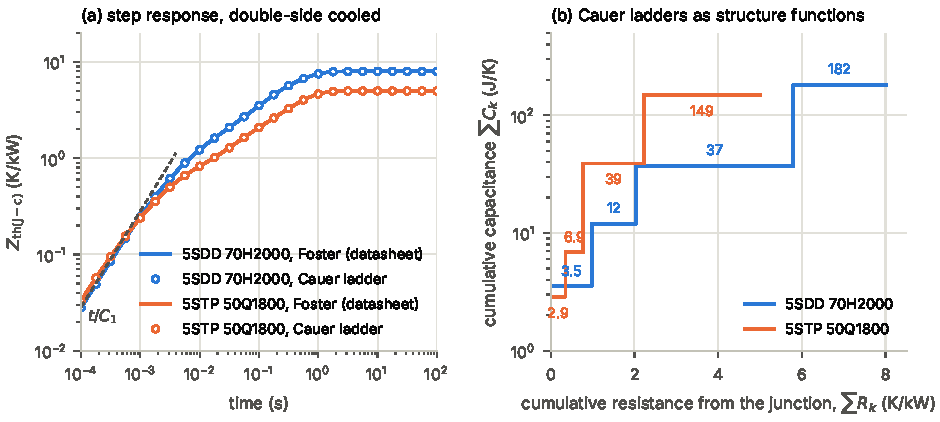
\includegraphics[width=\textwidth]{figures/fig_datasheet.pdf}
\caption{The two devices of Table~\ref{tab:cauer}. (a) Step response of the datasheet table (lines) and of the Cauer ladder (circles), double-side cooled; the dashed line is $t/C_1$ of the diode, the start of every network with this impedance. (b) The ladders as structure functions: cumulative capacitance against cumulative resistance from the junction, with the cumulative capacitance of each step.}
\label{fig:datasheet}
\end{figure}

\subsection{One ladder per side}
For the diode $\Rpar = \fcddRpar$~\KkW, $k_\mathrm{a} = \fcddKa$ and $k_\mathrm{c} = \fcddKb$, and \fcddShareA~\% of the heat leaves through the anode in steady state. The two ladders \eqref{eq:split} are in Table~\ref{tab:sides}; their single-side resistances are \fcddRsSuma{} and \fcddRsSumb~\KkW{} instead of \num{14.5} and \num{18.0}, because the table adds up to \fcddRth~\KkW{} and the parallel of the single-side values is \fcddRpar~\KkW. For the thyristor, with equal sides assumed, $k = 2$: each side is the ladder with doubled resistances and halved capacitances.

\begin{table}[htb]
\centering\small
\caption{Per-side ladders of the diode, \eqref{eq:split}. The junction capacitance $C_1 = \fcddCcA$~\JK{} is shared.}
\label{tab:sides}
\begin{tabular}{@{}l c c c c @{\hspace{1.5em}} c c c@{}}
\toprule
side & {$R_1k$} & {$R_2k$} & {$R_3k$} & {$R_4k$ (\KkW)} & {$C_2/k$} & {$C_3/k$} & {$C_4/k$ (\JK)} \\
\midrule
anode, $k_\mathrm{a} = \fcddKa$ & \fcddRsaA & \fcddRsaB & \fcddRsaC & \fcddRsaD & \fcddCsaB & \fcddCsaC & \fcddCsaD \\
cathode, $k_\mathrm{c} = \fcddKb$ & \fcddRsbA & \fcddRsbB & \fcddRsbC & \fcddRsbD & \fcddCsbB & \fcddCsbC & \fcddCsbD \\
\bottomrule
\end{tabular}
\end{table}

\subsection{The diode on two copper bars}
\label{sec:onbars}
To see what the ladder changes, the diode is clamped between two copper bars of \fccpCbar~\JK{} each (a bar $100 \times 10 \times \SI{180}{\milli\metre}$), lumped and adiabatic, through a contact of \fccpRch~\KkW{} per side, and dissipates \SI{\fccpP}{\kilo\watt} for \SI{\fccpT}{\second} (\SI{\fccpE}{\kilo\joule}). Three models of the device are compared (Fig.~\ref{fig:coupling}):
\begin{itemize}
\item the Cauer ladder split per side, each case on its contact and bar;
\item the Foster table with one case node, connected to both contacts and bars;
\item the Foster table on an ideal heat sink, for reference.
\end{itemize}
At the end of the pulse the junction has risen by \SI{\fccpTjC}{\kelvin} with the ladders, \SI{\fccpTjF}{\kelvin} with the Foster table on the bars and \SI{\fccpTjI}{\kelvin} on the ideal sink. The difference is the case. With the Foster table the whole power crosses the contacts from the first instant: the case jumps to \SI{\fccpTcFzero}{\kelvin} at once and ends at \SI{\fccpTcF}{\kelvin}. With the ladder, the heat into the bars starts from zero, reaches \SI{10}{\percent} of the power after \SI{\fccpQten}{\milli\second} and \SI{\fccpQend}{\percent} at the end of the pulse; \SI{\fccpEstored}{\kilo\joule} of the \SI{\fccpE}{\kilo\joule} (\SI{\fccpEstoredPct}{\percent}) are still in the device, and the warmer case has risen by \SI{\fccpTcC}{\kelvin}. After the pulse the stored heat flows into the bars and the junction cools more slowly than with the Foster table, which by then has already put all the energy into the bars.

The Foster table on the bars is not wrong in the direction of danger here, it is too pessimistic, by \SI{\fccpDiff}{\kelvin} on a margin computed against a junction limit; the ideal sink, at the other end, ignores the warming of the case. The ladder sits between them, close to the ideal sink for this pulse because little heat reaches the bars in half a second.

\begin{figure}[htb]
\centering
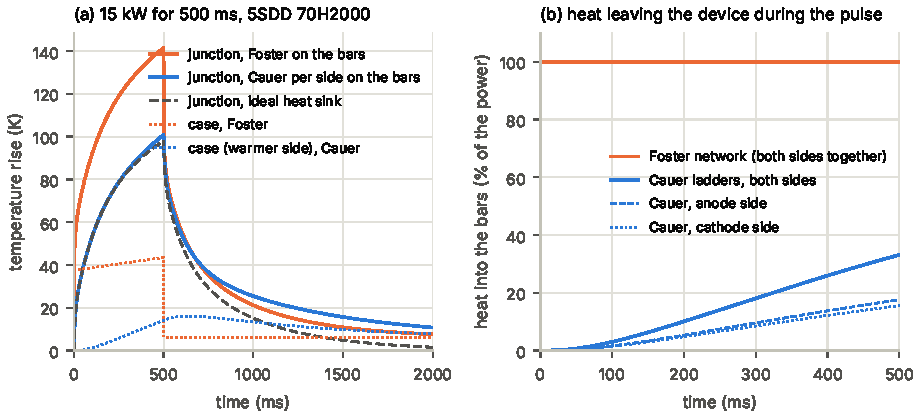
\includegraphics[width=\textwidth]{figures/fig_coupling.pdf}
\caption{Diode of Table~\ref{tab:cauer} between two copper bars (\fccpCbar~\JK{} and \fccpRch~\KkW{} contact per side), \SI{\fccpP}{\kilo\watt} for \SI{\fccpT}{\second}. (a) Junction and case temperature rise with the Cauer ladders per side, with the Foster table attached to the bars through one case node, and with an ideal heat sink. (b) Heat flowing into the bars during the pulse, as a share of the power.}
\label{fig:coupling}
\end{figure}

%=====================================================================
\section{Check against a press-pack with known layers}
\label{sec:synthetic}
The examples of Sec.~\ref{sec:examples} show the difference between the networks but not which is right, because the real device is not known. A synthetic press-pack is: a one-dimensional finite-difference model of the layers, whose exact transient impedance plays the role of the datasheet measurement and whose response on the bars plays the role of the truth.

\subsection{The model}
The device has the area of a \SI{63}{\milli\metre} pole and, from the anode case to the cathode case: copper pole \SI{8}{\milli\metre}, contact \SI{2.5}{\kelvin\per\kilo\watt}, molybdenum \SI{2}{\milli\metre} alloyed to the silicon, silicon \SI{0.5}{\milli\metre}, contact \SI{4}{\kelvin\per\kilo\watt}, molybdenum \SI{1.5}{\milli\metre}, contact \SI{2.5}{\kelvin\per\kilo\watt}, copper pole \SI{8}{\milli\metre}. Thermal conductivities \num{390}, \num{138} and \SI{120}{\watt\per\metre\per\kelvin}, volumetric heat capacities from the densities and specific heats of copper, molybdenum and silicon. The losses are spread evenly over the silicon and the junction temperature is the mean temperature of the silicon, as a virtual junction temperature would be. The model has \fcsyNodes{} cells; heat capacities: silicon \fcsyCsi, molybdenum \fcsyCmo, copper \fcsyCcu~\JK, together \fcsyCtot~\JK. With both faces held constant $\Rjc = \fcsyRth$~\KkW; anode side alone \fcsyRa, cathode side alone \fcsyRc~\KkW. A second variant has equal sides (the cathode side made like the anode side), to separate what comes from the split.

The exact impedance of the model is a Foster sum of its modes (\fcsyModes{} terms with a weight above $10^{-12}$ of the total, time constants from \SI{9}{\micro\second} to \SI{0.34}{\second}). Its exact ladder, from the bidiagonalization (the polynomial expansion returns negative elements here), gives back the impedance to $\fcsyErrFull$. As a datasheet would, the impedance is then sampled from \SI{1}{\milli\second} to \SI{10}{\second} and fitted with three to six Foster terms; the four-term fit is within \SI{\fcsyFitFourErr}{\percent} of the curve in the window.

\subsection{Structure function}
Figure~\ref{fig:synthetic}b shows the exact ladder as a structure function with the cumulative heat capacity of the layers. It follows them: a step of about \fcsyCsi~\JK{} for the silicon, the molybdenum, a flat part across the contacts, the steep rise of the copper; up to \SI{99}{\percent} of $\Rjc$ the cumulative capacitance is \fcsyCninetyNine~\JK{} against the \fcsyCtot~\JK{} of the layers. Then the curve goes vertical: the last resistance is held at constant temperature on the other side, which in the structure function is an infinite capacitance.

The ladders of the fits are coarse staircases of the same curve. Their total capacitance is \fcsyFitThreeCsum, \fcsyFitFourCsum, \fcsyFitFiveCsum{} and \fcsyFitSixCsum~\JK{} for three to six terms, a third to two thirds of the heat capacity of the layers. What is missing is the copper next to the faces. With the faces held constant that copper stays nearly at their temperature, stores little heat and hardly changes the curve, so a fit over the measured window does not see it; the more terms, the more of it the ladder recovers. The junction capacitance is the most robust number: \fcsyFitFourCo~\JK{} from four terms against \fcsyCsi~\JK{} of the silicon.

\begin{figure}[htb]
\centering
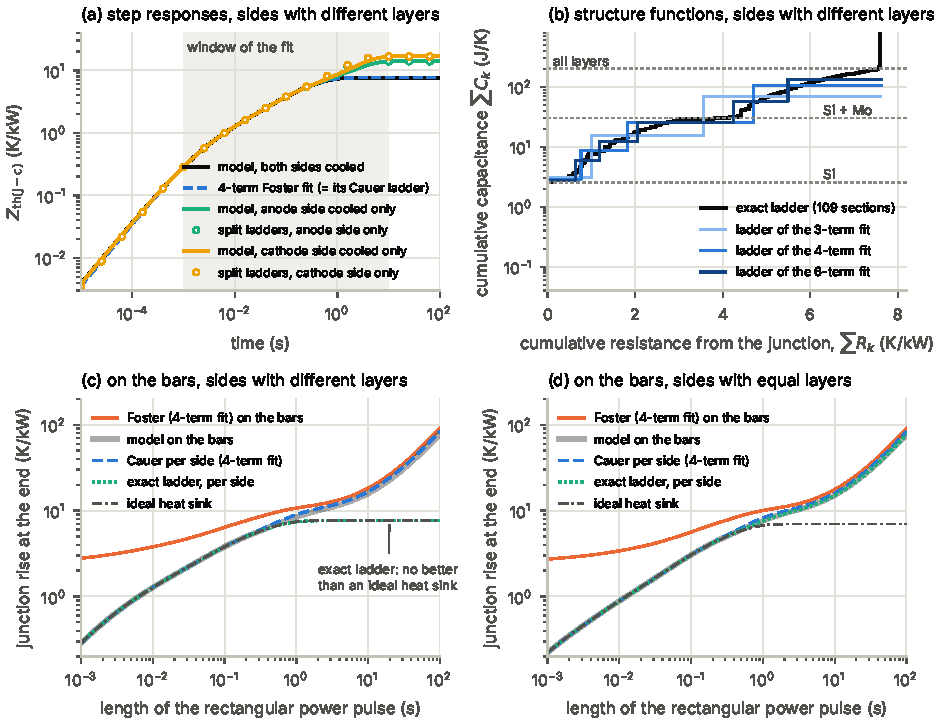
\includegraphics[width=\textwidth]{figures/fig_synthetic.pdf}
\caption{Synthetic press-pack. (a) Step responses of the model with both sides cooled and with one side only, the four-term fit over the window, and the single-side curves of the split ladders of that fit. (b) Exact ladder of the model and ladders of the fits as structure functions; dotted lines: cumulative heat capacity of the layers. (c), (d) Junction rise per kilowatt at the end of a rectangular pulse with the device between two bars (\fccpCbar~\JK, \fccpRch~\KkW{} per side): model, Cauer ladders per side, Foster table on the bars, ideal heat sink; (c) sides with different layers, (d) equal sides.}
\label{fig:synthetic}
\end{figure}

\subsection{On the bars}
The device is placed between the two bars of Sec.~\ref{sec:onbars} and the junction rise at the end of a rectangular pulse is compared with the model (Fig.~\ref{fig:synthetic}c and~d, Table~\ref{tab:synthetic}).

\begin{table}[htb]
\centering\small
\caption{Synthetic press-pack between two bars: junction rise per kilowatt at the end of a pulse of \SI{0.5}{\second}, its deviation from the model, and the largest deviation for pulses from \SI{1}{\milli\second} to \SI{100}{\second}.}
\label{tab:synthetic}
\begin{tabular}{@{}l c c c @{\hspace{1.5em}} c c c@{}}
\toprule
& \multicolumn{3}{c}{sides with different layers} & \multicolumn{3}{c}{equal sides} \\
\cmidrule(lr){2-4}\cmidrule(l){5-7}
& {\SI{0.5}{\second}, \KkW} & {dev., \%} & {largest, \%} & {\SI{0.5}{\second}, \KkW} & {dev., \%} & {largest, \%} \\
\midrule
model (truth) & \fcsyHalfZm & & & \fcssHalfZm & & \\
Cauer per side, 4-term fit & \fcsyHalfZc & \fcsyHalfEc & \fcsyMaxEc & \fcssHalfZc & \fcssHalfEc & \fcssMaxEc \\
Cauer per side, exact ladder & \fcsyHalfZx & \fcsyHalfEx & \fcsyMaxEx & \fcssHalfZx & \fcssHalfEx & \fcssMaxEx \\
Foster on the bars, 4-term fit & \fcsyHalfZf & \fcsyHalfEf & \fcsyMaxEf & \fcssHalfZf & \fcssHalfEf & \fcssMaxEf \\
ideal heat sink & \fcsyHalfZi & \fcsyHalfEi & & \fcssHalfZi & \fcssHalfEi & \\
\bottomrule
\end{tabular}
\end{table}

\begin{itemize}
\item The ladder of the four-term fit, split per side, follows the model within \SI{0.3}{\percent} for pulses up to \SI{0.1}{\second}, and is \SIrange{5}{7}{\percent} high for longer ones, with both variants: \fcsyMaxEc~\% at most with different sides, \fcssMaxEc~\% with equal sides. With three, five and six terms the largest deviation is \fcsyFitThreeDev, \fcsyFitFiveDev{} and \fcsyFitSixDev~\%: it shrinks as the ladder recovers the capacitance near the faces.
\item The Foster table on the bars is \SI{\fcsyHalfEf}{\percent} high at \SI{0.5}{\second} and much more for short pulses, when the junction rise is small and the contact drop of the full power is not: at \SI{10}{\milli\second} it is three to four times the model.
\item The ideal heat sink is right up to about \SI{0.1}{\second} and then increasingly low.
\end{itemize}

\subsection{What the ladder does not contain}
\label{sec:missing}
Three effects explain the deviations, and they are worth keeping in mind for any ladder from a datasheet.

\emph{Heat capacity near the case.} The test with the case held constant is insensitive to heat capacity close to the case, so the fitted ladder has less of it than the device. On a heat sink that warms up, that capacity would absorb heat; without it the junction comes out a few percent too warm. The error is on the safe side.

\emph{Single-side transients.} The same missing capacity weighs more when one face is adiabatic: the side that does not cool warms up as a whole, all its copper takes heat, and the ladder does not have that copper. The split ladders of the four-term fit give single-side curves up to \SI{\fcsySaDevF}{\percent} too high around \SI{\fcsySaDevT}{\second}, with equal sides as well (\SI{\fcssSaDevF}{\percent}); their steady state is right within the small difference between $\sum R_i$ and $\Rpar$. With the exact ladder of the equal-sided device the single-side curves are within \SI{\fcssSaAbsX}{\percent} of the model: the split itself is exact when the sides are proportional, and the error comes from the fit.

\emph{The exact ladder of different sides.} When the sides differ, the exact ladder of the double-side impedance is a single path that imitates two different ones. It follows the layers up to almost all of $\Rjc$ (Fig.~\ref{fig:synthetic}b) and then ends in sections with very small resistances and capacitances up to $\fcsyCmax$~\JK, which are not material. With the case held constant they are harmless. On the bars they act as a second heat sink: the junction follows the ideal-sink curve and is up to \SI{\fcsyMaxEx}{\percent} too cold for long pulses (Fig.~\ref{fig:synthetic}c), and its single-side curves stay far below the single-side resistances (\SI{\fcsySaDevX}{\percent} at \SI{50}{\second}). With equal sides the exact ladder has no such sections and follows the model within \SI{\fcssMaxEx}{\percent} (Fig.~\ref{fig:synthetic}d). A ladder from a fit of a few terms, as from a datasheet, does not develop the problem; a ladder from a fine structure-function analysis of a double-side measurement has to be cut where the structure function turns vertical before it is connected to anything.

Below the window of the fit the opposite holds: the network extrapolates the curve with the slope $t/C_1$, while a real device follows $\sqrt{t}$ \cite{activeclamping}. At \SI{100}{\micro\second} the four-term fit is \SI{\fcsyShortA}{\percent} from the model, at \SI{10}{\micro\second} \SI{\fcsyShortB}{\percent}: too low, on the unsafe side, for pulses shorter than the fastest time constant of the table.

%=====================================================================
\section{Procedure}
\label{sec:procedure}
\begin{enumerate}
\item Take the Foster table of $\Zjc$ from the datasheet, double-side cooled for a press-pack, and check that $\sum R_i$ equals the datasheet $\Rjc$. Note the time window of the curve: below it the table is an extrapolation.
\item Convert it with \code{foster\_to\_cauer()} (up to a dozen terms) or \code{foster\_to\_cauer\_bidiag()} (any number). Check that all elements are positive, that $\sum R_k = \sum R_i$, $C_1 = 1/\sum (R_i/\tau_i)$, $\sum C_k\theta_k^2 = \sum R_i\tau_i$, and that the round trip \eqref{eq:eig} gives back the table.
\item For a double-side cooled device whose sides see different external networks, split the ladder with the single-side resistances of the datasheet, \eqref{eq:split}. Without single-side values, take equal sides and say so.
\item Connect each case node to its external network: contact resistance per side, then the heat sink or the busbar model. Do not connect a Foster network to anything but a constant temperature.
\item Run the model once with the case nodes on a constant temperature: it must reproduce $\Zjc$.
\item Compute the losses from the current with the conduction parameters at the maximum junction temperature, inject them at the junction node, integrate.
\item Read the junction temperature with the limits of the ladder in mind: a few percent high on a heat sink that warms up, more for single-side cooling transients, too low for pulses shorter than the fastest time constant of the table.
\end{enumerate}

%=====================================================================
\appendix
\section{Companion scripts}
\label{sec:scripts}
\begin{itemize}
\item \code{foster\_cauer.py} is a module with the relations of the note, in SI units (K/W, s, J/K): the conversions \code{foster\_to\_cauer} (the function of Sec.~\ref{sec:code}, unchanged in its steps), \code{foster\_to\_cauer\_mp} (the same steps with \fcmpDigits{} digits, as reference), \code{foster\_to\_cauer\_bidiag} (Sec.~\ref{sec:bidiag}) and \code{cauer\_to\_foster} (Sec.~\ref{sec:inverse}); the step responses \code{zth\_foster} and \code{zth\_cauer}; the checks \code{invariants} and \code{ladder\_moment}; the split \code{split\_sides}; the staircase \code{structure\_function}; and a class \code{Network} that assembles nodes, ladders, contacts and heat sinks and computes their exact response to a piecewise-constant power from the eigenvalues of the network (nodes without capacitance are eliminated first). Run as a program it checks the three conversions against each other.
\item \code{foster\_cauer\_calc.py} holds the data of the examples at its top and produces the numbers and the figures of the note: the log \code{foster\_cauer\_results.txt}, the file \code{foster\_cauer\_values.tex} with every number quoted here as a macro, and \code{figures/*.pdf}. It runs in about twenty seconds. To convert another device, replace a table in \code{DIODE} or \code{THYR}; the external network of the examples is set by \code{R\_CH} and \code{C\_BAR}, the synthetic device by \code{LAYERS}.
\end{itemize}

%=====================================================================
\begin{thebibliography}{99}
\small
\item[] References marked [M] are quoted from memory: their bibliographic data, and the statements taken from them, have to be checked on the source before use in a design document. The datasheet tables were taken from the device datasheets as used in the thermal check the function was written for.

\bibitem{foster1924}
[M] R.~M.~Foster, ``A reactance theorem'', \emph{Bell System Technical Journal}, vol.~3, no.~2, pp.~259--267, 1924.

\bibitem{cauer1926}
[M] W.~Cauer, ``Die Verwirklichung von Wechselstromwiderst\"anden vorgeschriebener Frequenzabh\"angigkeit'', \emph{Archiv f\"ur Elektrotechnik}, vol.~17, pp.~355--388, 1926. Canonical ladder forms of driving-point impedances.

\bibitem{guillemin1957}
[M] E.~A.~Guillemin, \emph{Synthesis of Passive Networks}, Wiley, 1957. Properties of RC driving-point functions: alternation of poles and zeros, Foster and Cauer forms.

\bibitem{szekely1988}
[M] V.~Sz\'ekely, T.~Van~Bien, ``Fine structure of heat flow path in semiconductor devices: a measurement and identification method'', \emph{Solid-State Electronics}, vol.~31, no.~9, pp.~1363--1368, 1988.

\bibitem{szekely1997}
[M] V.~Sz\'ekely, ``A new evaluation method of thermal transient measurement results'', \emph{Microelectronics Journal}, vol.~28, no.~3, pp.~277--292, 1997. Time-constant spectrum, Foster--Cauer transformation and structure functions.

\bibitem{jesd5114}
[M] JEDEC, \emph{JESD51-14: Transient Dual Interface Test Method for the Measurement of the Thermal Resistance Junction to Case of Semiconductor Devices with Heat Flow Through a Single Path}, 2010.

\bibitem{golubkahan1965}
[M] G.~H.~Golub, W.~Kahan, ``Calculating the singular values and pseudo-inverse of a matrix'', \emph{SIAM Journal on Numerical Analysis, Series B}, vol.~2, no.~2, pp.~205--224, 1965.

\bibitem{paige1982}
[M] C.~C.~Paige, M.~A.~Saunders, ``LSQR: an algorithm for sparse linear equations and sparse least squares'', \emph{ACM Transactions on Mathematical Software}, vol.~8, no.~1, pp.~43--71, 1982. The lower bidiagonalization (\emph{Bidiag 1}) used in Sec.~\ref{sec:bidiag}.

\bibitem{gragg1984}
[M] W.~B.~Gragg, W.~J.~Harrod, ``The numerically stable reconstruction of Jacobi matrices from spectral data'', \emph{Numerische Mathematik}, vol.~44, pp.~317--335, 1984.

\bibitem{gautschi2004}
[M] W.~Gautschi, \emph{Orthogonal Polynomials: Computation and Approximation}, Oxford University Press, 2004. Conditioning of the map from moments to recurrence coefficients.

\bibitem{activeclamping}
pwr-control, \emph{Active clamping of high-voltage IGBTs: theory, design for a 6.5 kV / 1000 A module and a Simscape TVS model}, \texttt{research/power\_electronics/active\_clamping} of this repository: effective heat capacity $\bigl(\sum_i R_i/\tau_i\bigr)^{-1}$ of a Foster table and the $\sqrt{t}$ law at short times.

\end{thebibliography}

\end{document}
